\section{Lato Android}
Per quanto rigurda la fase di testing di quanto implementato per il client Android sono stati sfruttati principalmente due tool:
\begin{itemize}
	\item \textbf{Junit} per l'analisi dinamica del codice, con lo scopo, quindi di verificare che il codice scritto funzioni in maniera coerente a quanto richiiesto e che vengano seguiti le richieste descritte nei casi d'uso.
	\item \textbf{Espresso Junit} per l'analisi dell'interfaccia grafica costruita per la gestione delle varie richieste. Anche in questo caso si è fatto riferimento a quanto descritto dai casi d'uso riguardo alle view e al loro formato per osservare la correttezza di quanto implementato. 
\end{itemize}
\subsection{Espresso Junit}
Come detto, \textbf{Espresso Junit} è un tool attraverso il quale è possibile verificare le interazioni di un applicativo Android con l'utente. In questo caso, quindi, gli \textit{assert} verificano, ad esempio, che il fragment aperto sia quello corretto e che i campi dei vari componenti inseriti abbiano il valore desiderato.
\\ \noindent
Nell'ambito di questa iterazione, le componenti che sono state testate con questo applicativo sono:
\begin{enumerate}
	\item Login;
	\item Registrazione manuale di un libro;
	\item Ricerca di un libro.
\end{enumerate}
\noindent 
Consideriamo, come esempio per la descrizione, il test relativo alla ricerca di un libro all'interno della rete di Book Crossing. Il test si compone nel seguente modo:
\begin{lstlisting}
@Test
public void searchBookTestOK(){
	Globals.isLoggedIn = true;
	Globals.usernameLoggedIn = "A";
	onView(withId(R.id.navigation)).check(matches(isDisplayed()));
	onView(withId(R.id.book_search)).perform(click());
	onView(withId(R.id.book_search)).check(matches(isDisplayed()));
	
	ViewInteraction checkTitle = onView(withId(R.id.title_search));
	ViewInteraction checkAuthor = onView(withId(R.id.author_search));
	ViewInteraction checkBtnSearch = onView(withId(R.id.search_button));
	
	checkTitle.check(matches(isDisplayed()));
	checkAuthor.check(matches(isDisplayed()));
	checkAuthor.check(matches(isDisplayed()));
	
	checkTitle.perform(setTextInTextView(""));
	checkAuthor.perform(setTextInTextView(""));
	
	checkTitle.perform(setTextInTextView("questa storia"));
	checkBtnSearch.perform(click());
	
	onView(withId(R.id.books_found)).check(matches(isDisplayed()));
	onData(anything()).inAdapterView(withId(R.id.books_found)).
	atPosition(0).perform(click());
	onView(withText(containsString("BOOKABLE"))).
	inRoot(withDecorView(not(mainActivityActivityTestRule.getActivity().getWindow().
	getDecorView()))).check(matches(isDisplayed()));
\end{lstlisting}
\noindent Questo caso di test verifica che la ricerca di un libro svolta in maniera corretta garantisce la visualizzazione dei corretti \textit{fragment} e dei \textit{Toast} formattati in maniera corretta.
La medesima procedura è stata implementata per le altre componenti descritte precedentemente; il fatto di utilizzare questo tool consente di svolgere anche un'analisi dinamica del codice, dal momento che se ci fosse un errore, la successione grafica subirebbe un crash o mostrerebbe qualcosa di sbagliato facendo fallire il caso di test previsto.

\section{Lato Server}
	\subsection{Analisi Statica}
		\begin{figure}[h!]
			\centering
			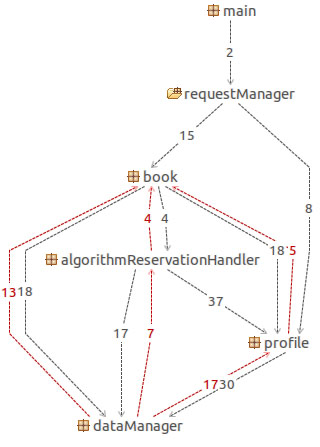
\includegraphics[width=0.3\textwidth]{Immagini/analisi_statica_package.jpg}
			\caption{Analisi statica del codice}
			\label{fig:analisiStatica}
		\end{figure}
		TODO:commentare immagine e controllare che corrisponda a quanto pianificato precedentemente
		
		
		Nel seguente piano sono rappresentate le metriche di:
		\begin{itemize}
			\item Abstractness: misura quanto facilmente il sistema può essere espanso;
			\item Instability: tentativo di misurare la facilità di cambiamento. 
		\end{itemize}
\newpage
	\begin{figure}[h!]
		\centering
		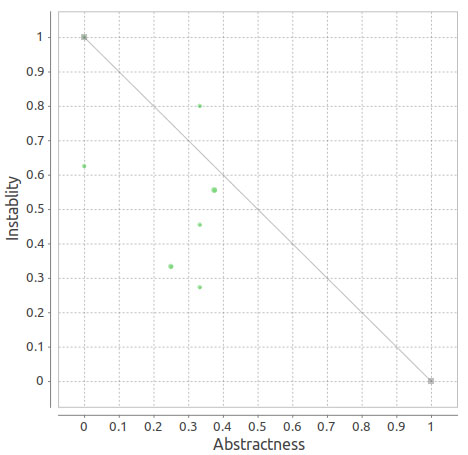
\includegraphics[width=0.3\textwidth]{Immagini/analisi_statica_grafico1.jpg}
		\caption{analisi statica grafico}
		\label{fig:analisiStaticaGrafico}
	\end{figure}		
	i packages vicino al punto (0,0) sono rigidi mentre i packages vicino a (1,1) sono totalmente astratti e quindi inutili, idealmente vorremmo trovarci sulla linea rappresentata.
	
	
	
	
	
	
	
